% LaTeX .tex example for the proceedings of
% COBEM 2017 - 24th International Congress of Mechanical Engineering
% December, 3-8, 2017, Curitiba, PR, Brazil
%
% Based on the template of the proceedings of COBEM2015 
% MODELO COBEM 2017

\documentclass[draft]{svjour3}

\usepackage{engsymbols}
\usepackage{magref}
\usepackage[utf8]{inputenc}
\usepackage{nicefrac}

\newcommand{\bmax}{\ensuremath{{B}\ped{max}}}
\newcommand{\bmin}{\ensuremath{{B}\ped{min}}}

\usepackage{mathptmx}
\journalname{Journal of the Brazilian Society of Mechanical Sciences and Engineering}

\usepackage{graphicx}
\usepackage{subfig}

\begin{document}

\title{Performance of Magnetic Refrigerators Operating with Different Magnetic Profiles}

\author{
Fábio P. Fortkamp \and
Gusttav B. Lang \and
Jaime A. Lozano \and
Jader R. Barbosa Jr.
}


\institute{
Fábio P. Fortkamp 
\at
POLO --- Research Laboratories for Emerging Technologies in Cooling and Thermophysics, Department of Mechanical Engineering, Federal University of Santa Catarina, Florianópolis, SC, 88040-900, Brazil, \email{fabio@polo.ufsc.br}
\and
Gusttav B. Lang \and
Jaime A. Lozano \and
Jader R. Barbosa Jr. \at POLO --- Research Laboratories for Emerging Technologies in Cooling and Thermophysics, Department of Mechanical Engineering, Federal University of Santa Catarina, Florianópolis, SC, 88040-900, Brazil}


\date{}


\maketitle

\begin{abstract}


\keywords{ magnetic refrigeration \and active magnetic regenerator \and numerical modeling \and magnetocaloric effect}
\end{abstract}

\section{Introduction}
\label{sec:introduction}

An active magnetic regenerator (AMR)  is a thermal regenerator composed of a solid porous matrix of magnetocaloric material, which changes its temperature according to the application of a varying magnetic field in synchronization with oscillatory fluid flows, due to the so-called magnetocaloric effect (MCE). Active magnetic regenerators are employed in magnetic refrigeration, a promising alternative to vapor compression systems due to its use of non-gaseous refrigerants and potentially higher  thermodynamic efficiency \cite{bib:trevizoli}. A magnetic refrigerator may contain multiple regenerator beds, in combination with rotary permanent magnets, to achieve higher levels of performance \cite{bib:trevizoli16_pump}. Since the working fluid only has energy transport functions and does not change its phase, aqueous solutions with freezing and corrosion inhibitors are usually employed.

The dynamic nature of AMR systems are described by two characteristic waveforms:

\begin{enumerate}
\item The \emph{magnetic profile}, which describes the time variation of the magnetic field experienced by the regenerators;
\item The \emph{fluid flow profile}, which describes the oscillatory flow rate though the regenerators
\end{enumerate}

Different combinations and arrangements of these waveforms yield different thermodynamic cycles through which an AMR system can operate. The most common cycle in the literature is the Brayton AMR cycle, which has two isentropic processes of instantaneous magnetization and demagnetization of the magnetocaloric material and two isofield processes \cite{bib:kitanovski}, as shown in Fig.~\ref{fig:brayton}. During magnetization, the solid material warms up due to the MCE; with a constant applied magnetic field, fluid flows, absorbing this energy and releasing it in the hot heat exchanger; the magnetic field is changed to a low level, cooling down the material; fluid from the hot source flows through the bed, releases its energy to the material, and the cold fluid can then absorb heat from the cold source. 

\begin{figure}[!ht]
  \centering
 %\includegraphics[width=5cm]{brayton-kitanovski}
  \caption{Temperature-entropy diagram for the Brayton AMR cycle, as experienced by the magnetocaloric (MC)  material \cite{bib:kitanovski}. The applied magnetic field is denoted by $H$.}
  \label{fig:brayton}
\end{figure}

The performance of AMR-based magnetic refrigerators is directly related to their thermodynamic cycle, and hence to the magnetic and fluid flow profiles. With this motivation, there are multiple studies in the literature regarding these waveforms. In general, the fluid flow profile is more easily changed in experimental prototypes with modifications in the hydraulic system, and it can be optimized for a given magnetic profile for higher cooling capacity or coefficient of performance \cite{bib:teyber17_exper,bib:nakashima18-influen-exp,FORTKAMP2018}. The actual shape of waveform depends on the hydraulic system configuration; single- or two-regenerators systems usually employ piston pumps with sinusoidal fluid flow profiles, while more complex valving system yield trapezoidal fluid flow profiles, with periods of no flow (when fluid is by-passed from the regenerator), periods with a constant flow rate and ramp transitions between these two states.


In room temperature magnetic refrigeration, the magnetic profile is generated by permanent magnets, representing the most expensive part of a magnetic refrigerator \cite{bib:bjoerk16_lifetime}, and hence considered fixed in AMR devices. Although the magnetic profile can be changed with motion control on the permanent magnets \cite{bib:benedict16_desig}, this is a topic yet to be better investigated, and most studies on the subject are numerical. The ideal Brayton cycle requires a instantaneous magnetic profile (square waveform), but in practice it is difficult to generate  stepwise variations of the magnetic field  using rotating permanent magnets arrays. Most magnetic refrigerators developed so far operate with a more continuous magnetic profile, such as the rectified cosine profile \cite{bib:tura-rowe-amr,bib:arnold14_desig,bib:trevizoli15_desig_halbac}, which is easily generated with compact devices and capable of achieving high levels of magnetic field \cite{bib:trevizoli16_pump}, but at the cost of  too brief demagnetization periods.

Many works on the analysis of  magnetic profiles use a ramp profile as  an approximation of the instantaneous profile with finite transition times between the magnetization levels, making it easier to generate the profiles with permanent magnets. The performance of an AMR subjected to a ramp magnetic profile and a instantaneous fluid flow profile with different parameters has been investigate \cite{bib:bjoerk11_amr}, but the emphasis was on the synchronization with the fluid flow profile and the authors did not compare different magnetic profiles. A study that  implemented different cycles through a ramp profile and a modification of the rectified cosine (consisting only of linear variations) \cite{bib:kitanovski} concluded that, with the same operating parameters parameters (temperature span between heat source and heat sink, frequency, mass flow rate, regenerator geometry, maximum applied magnetic field), the Brayton cycle (realized by a ramp profile) results in the highest cooling capacities; the same profile could be used in Ericsson cycles, with the magnetization processes done isothermally instead of adiabatically, and the result is higher values of the coefficient of performance. The conclusion that the instantaneous magnetic profile results in higher cooling capacities for a given temperature span, compared to other waveforms is also presented in \cite{bib:asme-mce}


In Fig.~\ref{fig:cycles}, the instantaneous and rectified cosine waveforms evaluated in this work are shown in terms of the average applied magnetic field (${B}$) that acts on the regenerator (vertical axis) for one AMR cycle parameterized in a time variable ($t$) ranging from 0 to the cycle period $\tau$ (horizontal axis).  

\begin{figure}[!ht]
  \centering
  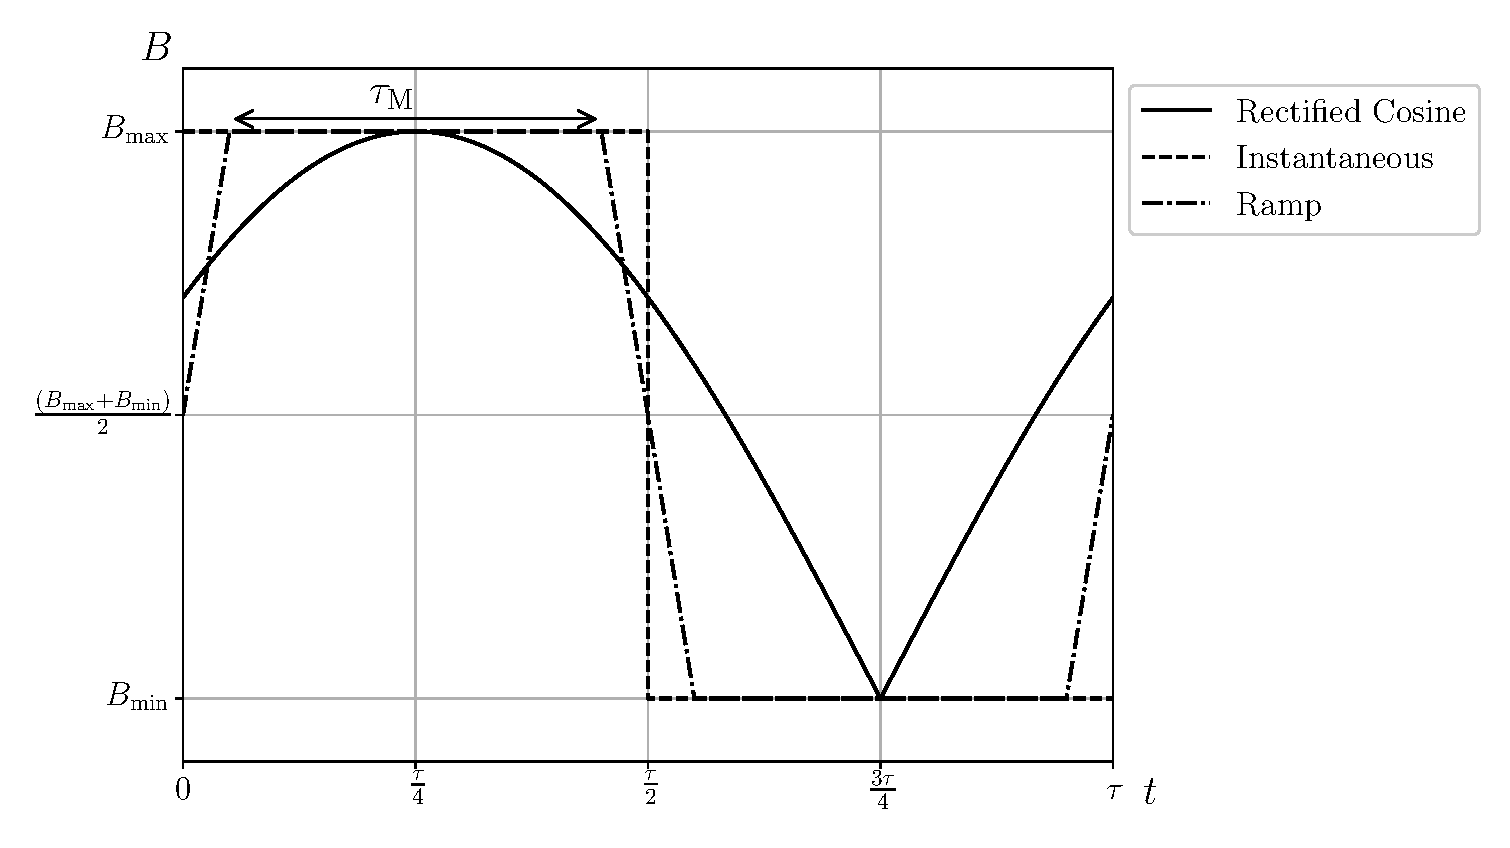
\includegraphics[width=7cm]{profiles_all.eps}
  \caption{Instantaneous and rectified cosine magnetic profiles in terms of the average magnetic field over the regenerator for one AMR cycle as a function of time ($t$). }
  \label{fig:cycles}
\end{figure}


The present work extends these analyses and attempts to systematically compare the performance of a magnetic refrigerator operating with instantaneous, rectified cosine and ramp magnetic  profiles under different parameters, with the goal of selecting the best magnetic profile for certain requirements of cooling capacity of a target application. In comparison with the previously cited works, we analyze the effect of different regenerator geometries and different levels of the magnetic field and mass flow rate. In particular, in comparison with the work of \cite{bib:kitanovski}, where the authors studied different combinations of flow and magnetic profiles to yield various thermodynamic cycles, we fix the fluid flow profile to better investigate the effect of the magnetic profile, which is used in the design of magnetic circuits.

\section{NUMERICAL SIMULATIONS}
\label{sec:numer-simul}

Simulations were performed using a one-dimensional AMR mathematical model \cite{bib:asme-mce,bib:trevizoli16_perfor_model}. The simulated magnetic refrigerators are composed of multiple prismatic regenerators filled with gadolinium (Gd) spheres as the magnetocaloric solid matrix, with the parameters shown in Table~\ref{tab:params}. The fluid is a mixture of water and ethylene glycol, in the proportion of \SI{80}{\percent}-\SI{20}{\percent} in volume.

\begin{table}[!ht]
  \centering
  \caption{Geometric and operation parameters for the simulated AMR devices}
  \begin{tabular}{c|c}
\hline
    \textbf{Parameter}&\textbf{Value}\\
\hline
Regenerator height & \SI{20}{\mm}\\
Regenerator width & \SI{25}{\mm}\\
Regenerator length & \SI{100}{\mm}\\
Number of regenerators & \num{11} \\
Particle diameter & \SI{0.5}{\mm}\\
Hot source temperature & \SI{298}{\kelvin}\\
Cold source temperature & \SI{278}{\kelvin}\\
\hline
  \end{tabular}
  \label{tab:params}
\end{table}

The AMR model solves mass and energy conservation equations for the solid and the fluid domains in an active magnetic regenerator. In this work, regenerators were assumed to be adiabatic to the environment. All beds experience the same flow and magnetic profiles, as detailed in the following sections.

\subsection{Flow profile}
\label{sec:flow-profile}


The flow profile through a given bed, i.e. the mass flow rate as a function of time $\rate{m}\ped{f} (t)$, is assumed to be a square wave as that shown in Fig.~\ref{fig:mprofile}. The cold blow has a duration of $\tau\ped{CB}$ and the  hot blow a duration of $\tau\ped{HB}$, while the period of one AMR cycle is $\tau$. Limiting the blow times during each half-cycle to periods where the magnetic field is at its maximum and minimum can result in increased performance \cite{bib:nakashima17_avaliac}. In this work, the blows are supposed to be in balance, thus, $\tau\ped{CB} = \tau\ped{HB}$. An important parameter regarding the flow profiles can be defined, which is the blow fraction, $F\ped{B}$:

\begin{equation}
  \label{eq:1}
  F\ped{B} = \frac{\tau\ped{CB} + \tau\ped{HB}}{\tau}
\end{equation}

\begin{figure}[!ht]
  \centering
%  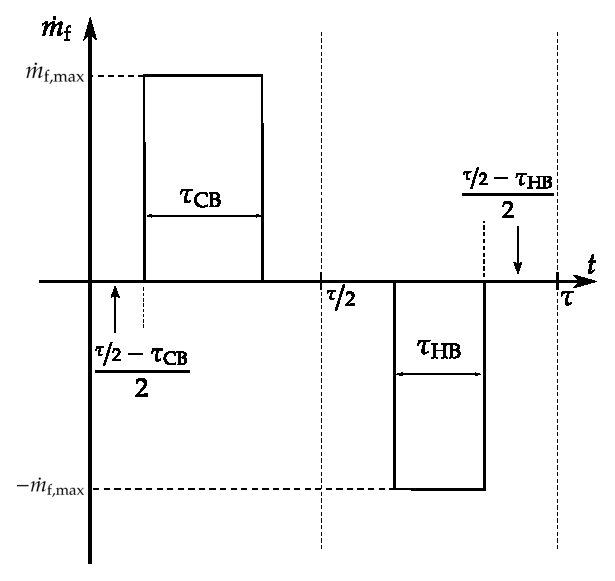
\includegraphics[width=7cm]{mprofile}
  \caption{Instantaneous flow profile used in the numerical simulations. "Positive" mass flow rate indicates flow in the direction from the cold to the hot source, and negative values represent the opposite direction. }
  \label{fig:mprofile}
\end{figure}

\subsection{Magnetic profile}
\label{sec:magnetic-profile}

The AMR mathematical model takes the magnetic profile as an input, and the profiles represented in Fig.~\ref{fig:cycles} were tested with different parameters. The mathematical definitions for the magnetic profiles over a cycle of period $\tau$ are as follows; the instantaneous profile (represented by the index ``I'') and the rectified cosine profile (represented by ``RC'') are defined solely in terms of the extrema values $\bmax$ and $\bmin$:

\begin{equation}
\average{B}\ped{I}(t)=
\begin{cases}
\average{B}\ped{max}, & 0 \le t < \nicefrac{\tau}{2} \\
\average{B}\ped{min}, & \nicefrac{\tau}{2} \le t < \tau\\
\end{cases}
\label{eq:4}
\end{equation}

\begin{equation}
\average{B}\ped{RC}(t) = \bmin + \left(\bmax - \bmin\right)  \left\lvert \cos\left( \frac{\pi}{\tau} \left( t - \frac{\tau}{4}\right)\right) \right\rvert
\label{eq:5}
\end{equation}


In this work, the average values of the magnetic field during each half-AMR cycle are considered for comparison between profiles. The average magnetic profile during the hot cycle ($0 \le t < \nicefrac{\tau}{2}$) is denoted $B\ped{h}$ and the average during the cold cycle  ($ \nicefrac{\tau}{2} \le t < \tau$) is denoted $B\ped{l}$.

\subsection{AMR operating parameters}
\label{sec:amr-oper-param}


Different numerical simulations were carried with different operating parameters such as: AMR cycle frequency ($f$), blow fraction ($F\ped{B}$) and utilization ($\Phi$) which is defined as:

\begin{equation}
\Phi = \frac{\rate{m}\ped{f,max}F\ped{B}\frac{\tau}{2}c_{p,\mathrm{f}}}{m\ped{s} c\ped{s}}
\label{eq:2}
\end{equation}

\noindent where $c_{p,\mathrm{f}}$ is the constant-pressure specific heat for the fluid, and $m\ped{s}$ and $c\ped{s}$ are the mass and specific heat of the solid phase in one bed. 

\section{RESULTS AND DISCUSSIONS}
\label{sec:results-discussions}

\subsection{Comparison of the instantaneous and rectified cosine profiles}
\label{sec:comp-inst-cosine}

When comparing the magnetic profiles, the average magnetic field during the hot cycle is the same; this implies in a higher peak for the rectified cosine. For the cold cycle, there are two possible comparison methods:

\begin{enumerate}
\item The minimum values for both profiles is the same;
\item The average value for both profiles during the cold cycle is the same.
\end{enumerate}

As a reference, in all simulations  the minimum value for the rectified cosine was fixed at $\average{B}\ped{min,RC} = \SI{0.1}{\tesla}$. For the first comparison, the minimum value for the instantaneous value was kept at the same level ($\average{B}\ped{min,I} =  \average{B}\ped{min,RC}$), hence, the average low value for the RC profile was higher ($B\ped{l,RC} > B\ped{l,I}$). Although this does not seem a fair comparison, in practice it is feasible to generate a profile with a constant low-valued plateau for the magnetic field \cite{bib:insinga16_optim,bib:benedict16_desig}. For the other comparison method, the low level of the instantaneous profile was increased ($\average{B}\ped{min,I} >  \average{B}\ped{min,RC}$) to keep the average the same ($B\ped{l,RC} = B\ped{l,I}$). In addition, simulations were ran for various values of blow fraction and the optimal cases were selected; the rectified cosine profile can benefit from a smaller blow fraction because this can concentrate the flow during the periods of very high or low fields. In this section, all results show the resulting optimal case of the blow fraction for each profile (for the values tested): fluid flowing during the entire period for the instantaneous profile, and only during \SI{60}{\percent} of the period for the cosine profile.


Figure~\ref{fig:cos_ins} shows the cooling capacity attained by the device at a frequency of \SI{1}{\hertz} and different utilizations, for both comparison methods.  The horizontal axis shows the average value during the high field region. Notice how the results are conflicting; for Fig.~\ref{fig:comp_min}, the instantaneous profile almost always yields a higher performance, while for Fig.~\ref{fig:comp_avg} the rectified cosine profile generates higher cooling capacities. Since the average during the hot cycle (high field stage) is the same, the main difference is due to the low magnetic field levels. For the ``same minimum'' comparison, the instantaneous profile is capable of keeping the magnetic field at low levels for the whole half-cycle, which is beneficial for performance;  for $\Phi=1.0$ and $B\ped{h} = \SI{1.40}{\tesla}$, the cooling capacity for the instantaneous profile is $\SI{196.3}{\percent}$ higher than for the cosine profile.  As demonstrated by \cite{bib:asme-mce}, a higher average magnetic field during the low-field stage increases the solid temperature and consequently results in  warmer fluid entering the cold heat exchanger, representing a thermal loss. In the ``same-average'' comparison, the cosine profile is capable of achieving much lower levels (since its minimum value is fixed), therefore providing more cooling power. However, as explained before, it is possible to design near-instantaneous profiles with very low levels of the magnetic field.


\begin{figure}[!ht]
  \centering
%  \subfloat[Same minimum]{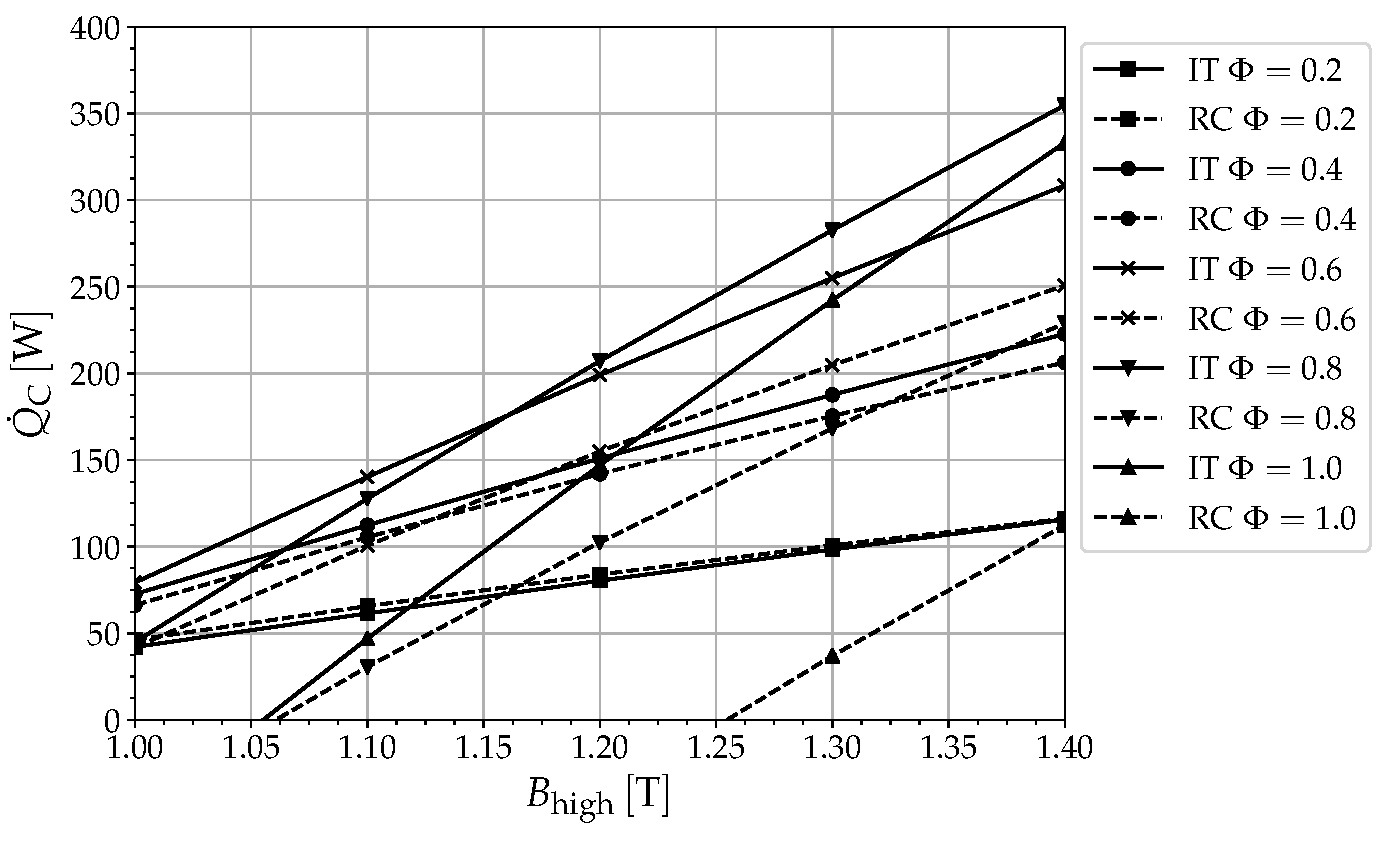
\includegraphics[width=8cm]{Qc_B_comp_f_1_same_minimum}\label{fig:comp_min}}
\,
%  \subfloat[Same average]{\includegraphics[width=8cm]{Qc_B_comp_f_1_same_low_average}\label{fig:comp_avg}}
\,
  \caption{Cooling capacity as a function of the  average high magnetic field, for different utilizations. “I”: instantaneous (blow fraction of \SI{100}{\percent}); “RC”: rectified cosine  (blow fraction of \SI{60}{\percent}), for both comparison methods.}
 \label{fig:cos_ins}
\end{figure}

The only exception in the ``same minimum'' comparison is seen for the lowest utilization of $\Phi = 0.2$, where the performance is slightly better for the RC profile. Since the blow fraction for the cosine is lower, the mass flow rate must be higher to yield the same utilization (cf. Eq.~\eqref{eq:2}), and this increases heat transfer rate, as previously explained ---  outweighing the effects of the magnetic field.

In general, the performance of the AMRs operating with the instantaneous magnetic profile yields better results. As can be seen on Fig.~\ref{fig:cos_ins}, an instantaneous profile with the lowest possible value of $\bmin$ and the highest possible value of $\bmax$, with a flow profile occupying the whole cycle with average values of utilization, results in the highest values of cooling capacity among all simulations, therefore, representing the ideal magnetic profile for an AMR.

\subsection{Analysis of the instantaneous profile}
\label{sec:deta-analys-inst}

As shown in the previous section, the instantaneous profile yields the highest values for cooling capacity. Therefore, in this section, a more detailed analysis of such profile has been carried out. Figure~\ref{fig:qc_phi_inst} shows the cooling capacity as function of utilization, for several levels of the maximum magnetic field for the instantaneous profile, for two different operating frequencies. Because of the conflicts between a low heat transfer rate for flow rates too low and a loss in regenerator effectiveness in flow rates too high, there are critical values of utilization that maximize cooling capacity, and this critical value grows with the level of magnetic field. With higher magnetic field, the increase in the MCE surpasses the loss of effectiveness, and one can go to higher flow rates without losing performance. It can also be seen in Fig.~\ref{fig:qc_phi_inst} that at higher frequencies, the values of cooling power are higher, and also the critical values of utilization are lower; however, this usually is achieved at the cost of higher power consumption in AMR devices at higher frequencies \cite{bib:lei15_study,NIKNIA2016601}.

\begin{figure}[!ht]
  \centering
\subfloat[$f = \SI{1}{\hertz}$]{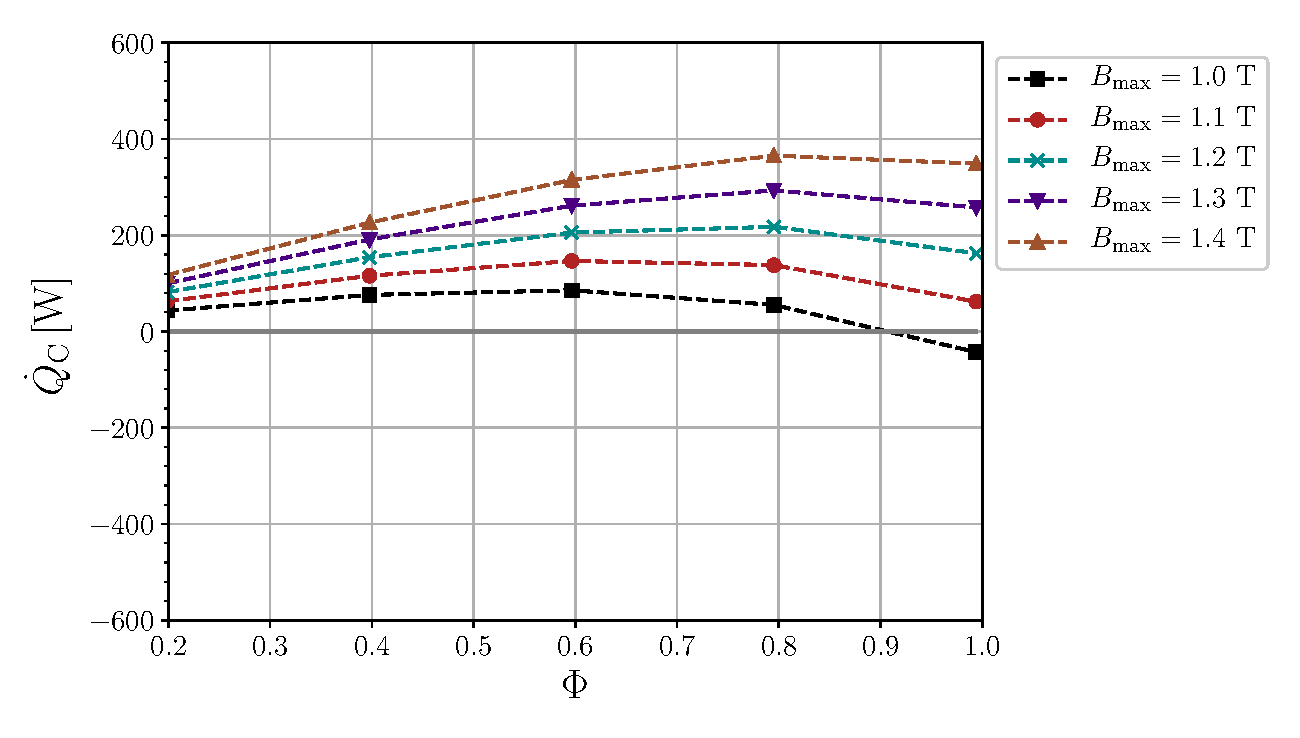
\includegraphics[width=8cm]{Qc_Phi_inst_f_1_Hmin_005_FB_100}\label{fig:Qc_phi_inst_1}}
\,
  \subfloat[$f = \SI{2}{\hertz}$]{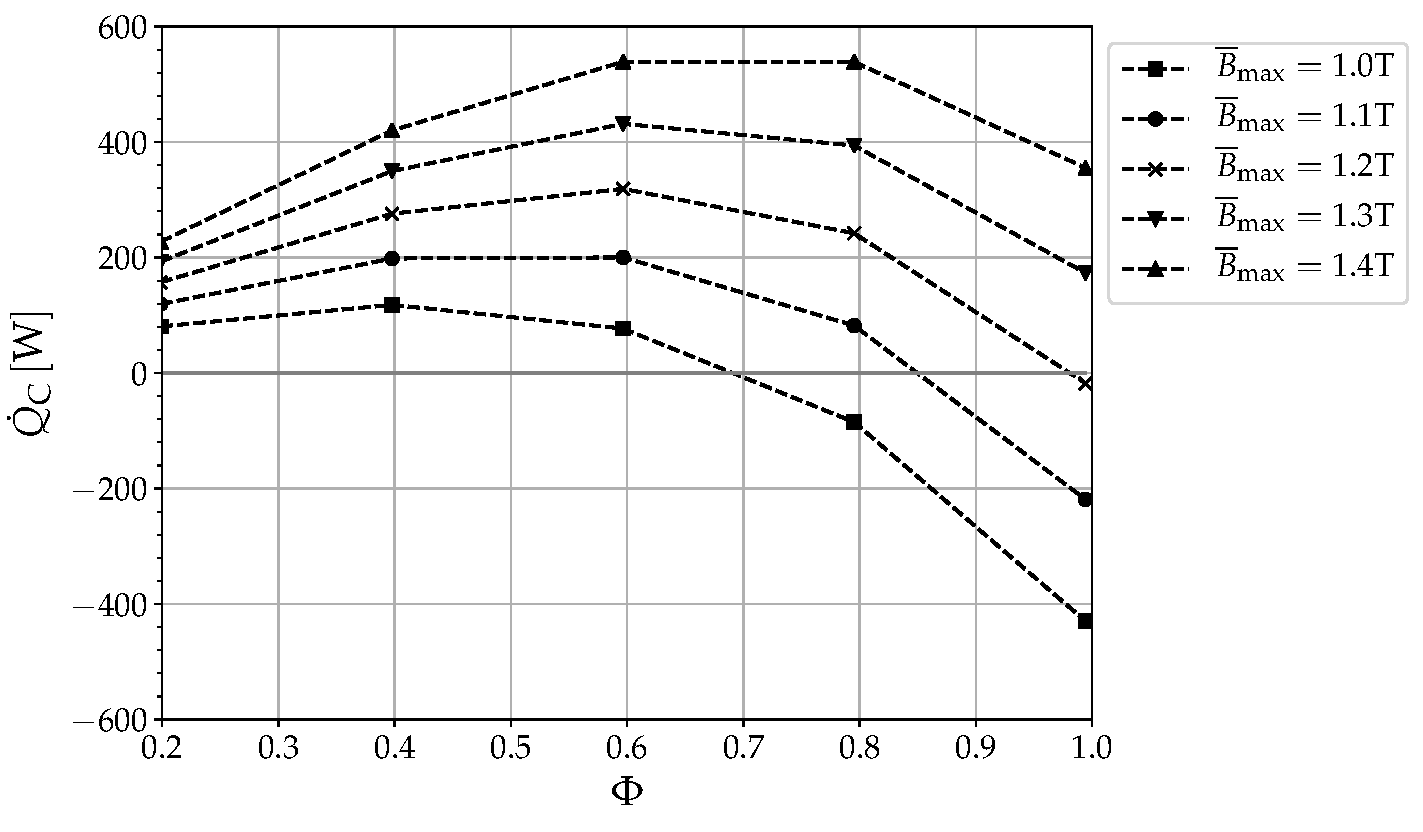
\includegraphics[width=8cm]{Qc_Phi_inst_f_2_Hmin_005_FB_100}\label{fig:Qc_phi_inst_2}}
  \caption{Cooling capacity as a function of utilization, for various values of the high magnetic field  of the instantaneous profile}
  \label{fig:qc_phi_inst}
\end{figure}

\begin{figure}[!ht]
  \centering
  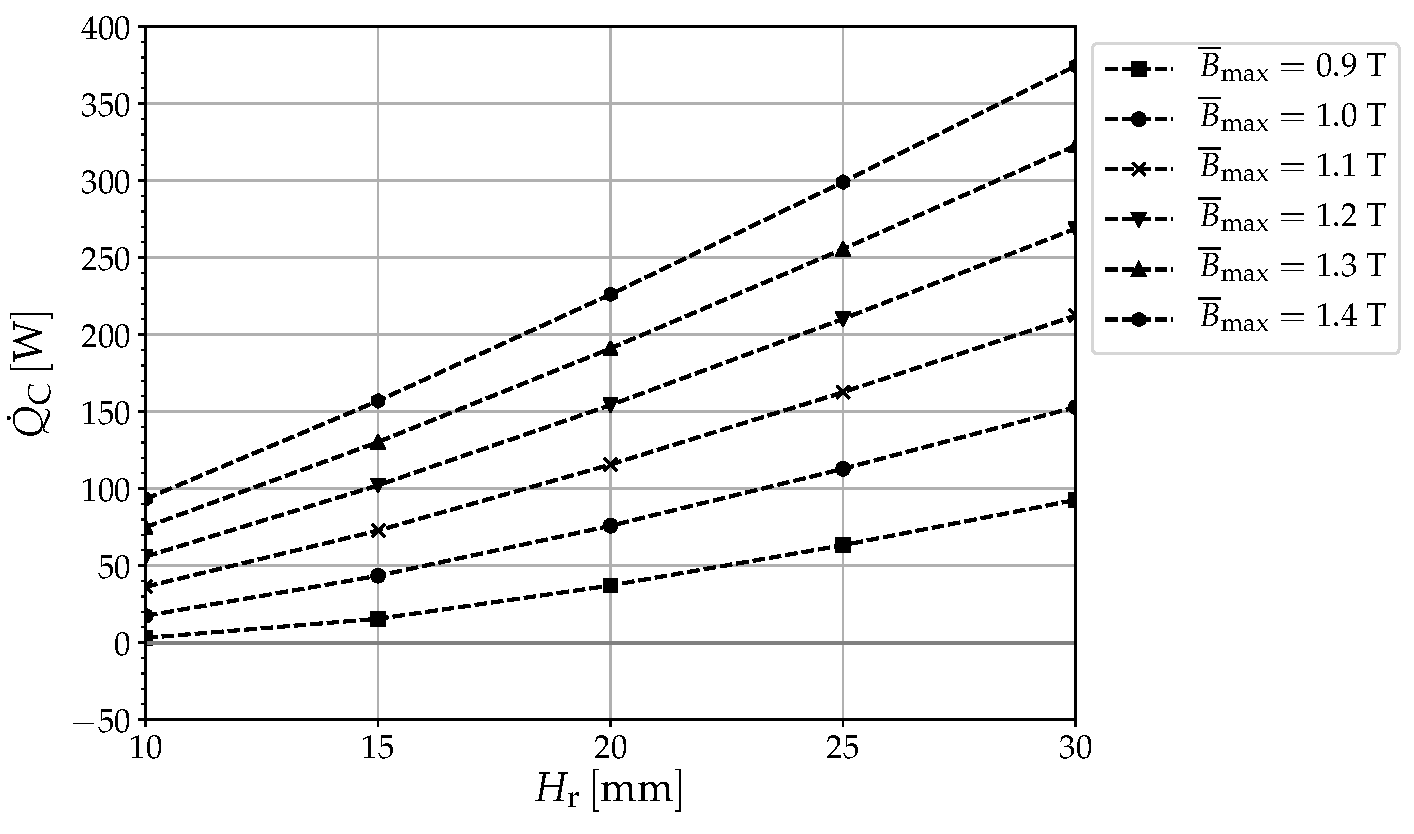
\includegraphics[width=8cm]{Qc_H_inst_f_1_Phi_40}
  \caption{Cooling capacity as a function of  regenerator height (all other parameters from Table~\ref{tab:params} constant) for various values of the high magnetic field of the instantaneous profile}
\label{fig:Qc_H_inst}
\end{figure}

The parameters in Table~\ref{tab:params} were chosen from preliminary simulations, but they are not guaranteed to be the optimal choices. To understand the impact of regenerator geometry on the performance with the instantaneous profile, the regenerator height was varied in Fig.~\ref{fig:Qc_H_inst}, and all other parameters from Table.~\ref{tab:params} were kept fixed. As expected, higher magnetic fields allow for smaller regenerators (and hence more compact systems). For instance, to achieve a capacity of \SI{100}{\watt}, increasing the field from \num{1.0} to \SI{1.2}{\tesla} result in using regenerators \SI{36}{\percent} smaller.

\section{CONCLUSIONS}
\label{sec:conclusions}

A one-dimensional AMR numerical model was used to compare the performance of a magnetic refrigerator under different operating and geometric parameters and with the instantaneous and rectified cosine magnetic profiles. Most of the AMRs operating with an instantaneous magnetic profile have resulted in better performances than those with a cosine profile, except in cases of low utilization. Although the cosine profile reaches higher levels of the magnetic field, the instantaneous profile can keep the magnetization (and demagnetization) for a longer period, which is shown to be beneficial to performance. Further analysis of the instantaneous profile has shown that the use of the highest possible value of the maximum magnetic field allows for using smaller regenerators and lower utilization, without losing performance.

\begin{acknowledgements}
This work was supported by CNPq, Embraco and EMBRAPII Unit Polo/UFSC.  
\end{acknowledgements}

% BibTeX users please use one of
%\bibliographystyle{spbasic}      % basic style, author-year citations
%\bibliographystyle{spmpsci}      % mathematics and physical sciences
\bibliographystyle{spphys}       % APS-like style for physics

\bibliography{thermo-ref/Thermo-Foam-Ref,thermo-ref/thesis}

\end{document}

%%% Local Variables:
%%% mode: latex
%%% TeX-master: t
%%% End:
